\clearpage
\section{Chování výrobce – krátkodobá rovnováha firmy, dlouhodobá rovnováhy firmy, bod
zvratu, bod zastavení činnosti firmy, odvození individuální nabídky.}

\subsection{Krátkodobá rovnováha firmy}
\begin{itemize}
    \item \textbf{Rovnováha} - stav, kdy aktéři, tvořící trh, nemají žádné důvody měnit
    své ekonomické chování. U firmy nastane při maximálním zisku.
    \item Platí $MC=MR$
\end{itemize}

\subsection{Dlouhodobá rovnováha firmy}
\begin{itemize}
    \item na trzích se prosazuje tendence k nulovému ekonomickému zisku
    \item Kladný ekonomický zisk firem je přechodnou situací.
\end{itemize}

\subsection{Bod zvratu}
\begin{itemize}
    \item Break Even Point
    \item množství produkce, od kterého začíná firma vytvářet zisk
    \item vyrovnání nákladů s příjmy
\end{itemize}

\subsection{Bod zastavení činnosti}
\begin{itemize}
    \item objem produkce, při kterém příjem nepokrývá ani variabilní náklady
    \item Je ekonomičtější nevyrábět vůbec, protože bude docházet k menším ztrátám 
    (ty budou rovné fixním nákladům)
\end{itemize}

\subsection{Odvození individuální nabídky}
Křivka individuální nabídky kopíruje část křivky mezních nákladů nad průsečíkem 
s~průměrnými variabilními náklady.

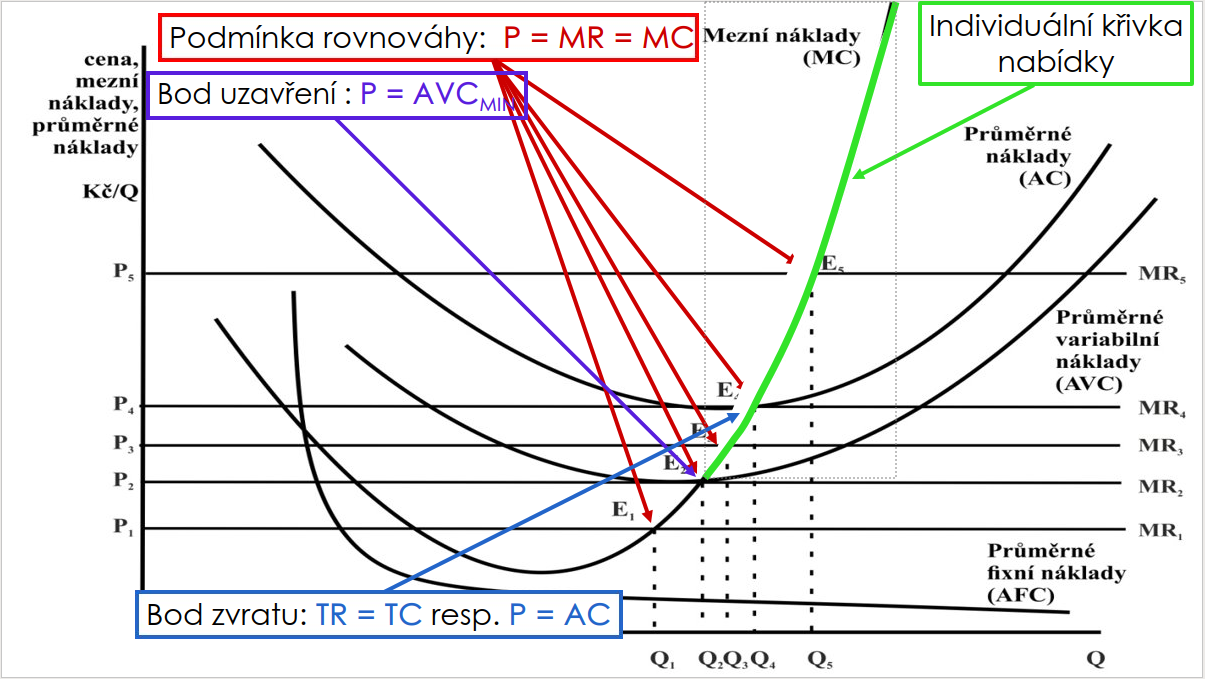
\includegraphics[width=16cm]{images/09_indiv_nabidka.png}